\subsection{Retrieving single source position in free field}

The purpose of this experiment is to test the sound localization algorithms in a controlled environment. A tetrahedral array receives sound waves emitted by a point source and its location is  retrieved. The point source position is fixed and the microphone array is rotated around its axis in order to change the relative source location (azimuth). A diagram of the setup is display in figure \ref{fig:Anechoic1} where the two point source position are shown: 90 and 30 degree.  The source is pink noise, but a recording of 300Hz sinusoidal wave is also performed to display the between the microphones (Fig. \ref{fig:pinknoise}). In order to recreate the far field conditions in the limited space of the anechoic chamber, the array is placed as far away from the source as possible and the array aperture is reduced to approximate plane wave propagation better. 

\begin{figure}[H]
    \centering
    \includegraphics[width=0.7\textwidth]{Figures/Anechoicexp1.png}
    \caption{Diagram of the experiment}
    \label{fig:Anechoic1}
\end{figure}
 

\subsubsection{Stimuli and settings}

The source is a Brüel \& Kjær Omnisource type 4296 with operating frequency of 100 to 5000 Hz. Brüel \& Kjær PULSE system is used to record the sound picked up by the microphone array. The sampling frequency is set at 131072Hz which is the highest sampling frequency available on the PULSE system. Temperature of the lab is recorded at 22 $\degree$. The prototype microphone array allows adjustment of the aperture size between 10cm-1m. The aperture is reduced to 0.395m.
%When strong periodicity in the signal, the array can in theory work with waves of frequency up to 874 Hz before aliasing occurs. In our case there is no strong periodicity when we are using pink noise as sound sources, much higher frequencies can be input \ref{REF}.

%\begin{equation}
%    f=\frac{c}{\lambda}=\frac{345}{0,395} \approx 874 (Hz)
%\end{equation}

 
\subsubsection{Delay between the microphones}
 
 In order to verify the accuracy of the measurements, sample delay is measured at a single frequency. In order to avoid the pressure field frequency zone of the anechoic chamber and array aliasing, 300 Hz sin wav is used. 
 %A single frequency is chosen to avoid group delay issues.  
 
 \begin{figure}[H]
    \centering
    \includegraphics[width=0.8\textwidth]{Figures/delaytetra300Hz.png}
    \caption{Sin wave recorded by the four microphones.}
    \label{fig:pinknoise}
\end{figure}
 
 
\begin{center}
  \begin{tabular}{ | l | c | r | r | r |}
    \hline
    Delays & Mic 1 & Mic 2 & Mic 3 & Mic 4 \\ \hline
    Mic 1 & X & -6&114 & 52  \\ \hline
    Mic 2 &   & X &120 & 58  \\ \hline
    Mic 3 &   &   & X  &-61  \\ \hline
    Mic 4 &   &   &    & X   \\ \hline
  \end{tabular}
  \captionof{table}{Sample delay measured between the microphones at 0 incidence (Fs= 131072Hz)}
\end{center}

%Variation in delay are due to the source position inaccuracies or could be due to the plane wave approximation not holding. Therefore wider peaks are to be expected and a slight shift from the zero degree position. The microphones are not calibrated in this experiment as we can see difference in amplitude are noticeable.
 
\subsubsection{Results}

Wave files recorded by the pulse system are used by the algorithm. The script "NAMEOFTHESCRIPT" is run and the energy maps of the SRP-PHAT and minimum power SRP-PHAT algorithms are computed and displayed in the following part.


\begin{figure}[H]
    \centering
    \begin{subfigure}[b]{0.96\textwidth}
    \centering
    \includegraphics[width=0.95\textwidth]{Figures/Anechoic0Deg1SrcNorm.png}
\end{subfigure}
\vskip \baselineskip
\begin{subfigure}[b]{0.96\textwidth}
    \centering
    \includegraphics[width=0.95\textwidth]{Figures/Anechoic0Deg1SrcMinPow.png}
\end{subfigure}
\caption{Figures depict from top-to-bottom SRP-PHAT and minimum power SRP-PHAT localization for source around (90 $\degree$, 0$\degree$) in the Anechoic Room}
\end{figure}

 The source is localized slightly above 0$\degree$ elevation. This is because the top microphone of the array was on the same horizontal axis as the acoustic center of the sound source. 
%This shift can also be explained by the inaccuracies in the microphone positions on the microphone array. The prototype microphone array allows the 3 microphones on the horizontal axis to move up and down in order to adjust the microphone array aperture relative to the "fixed" top microphone. Therefore there might be a maladjustment in the position of the 3 lower microphones relative to the top microphone thus creating an incorrect position on the vertical axis and ultimately an error in the localization. 
The height of the microphone array is later increased in order to place the 3 lower microphones on the same vertical axis as the acoustic center of the sound source. The following figure shows the results for source at (30 $\degree$, 0$\degree$). 
%This could also be due to a tilt of the array or the source not being in the far-field.
%As will be seen in the following graphs of the sound source at 30 $\degree$ azimuth the elevation error is reduced. No further investigation are done. 

\begin{figure}[H]
    \centering
    \begin{subfigure}[b]{0.96\textwidth}
    \centering
    \includegraphics[width=0.95\textwidth]{Figures/Anechoic30Deg1SrcNorm.png}
\end{subfigure}
\vskip \baselineskip
\begin{subfigure}[b]{0.96\textwidth}
    \centering
    \includegraphics[width=0.95\textwidth]{Figures/Anechoic30Deg1SrcMinPow.png}
\end{subfigure}
\caption{Figures depict from top-to-bottom SRP-PHAT and minimum power SRP-PHAT localization for source at 30 degree}
\end{figure}

\newpage
\subsection{Retrieving the multi-sources location and relative level in free field}

This experiment is run in the anechoic chamber with focus on retrieving the relative source level difference of two sources playing at the same time. One source is placed at (90$\degree$, 0$\degree$) and plays a pink noise at 46dBA, the second source is placed at (130$\degree$, 0$\degree$) and plays an uncorrelated pink noise at 52dbA. Two custom spherical speakers are used to play the source signal and the aperture size of the array is 0.395m. The files are generated in MATLAB and low frequencies (<200Hz) are filtered out in order to accommodate for the speaker used.  The sound from each speaker is measured individually using a level meter in order to check the playback levels. Temperature of the room is 22$\degree$C.

\begin{figure}[H]
    \centering
    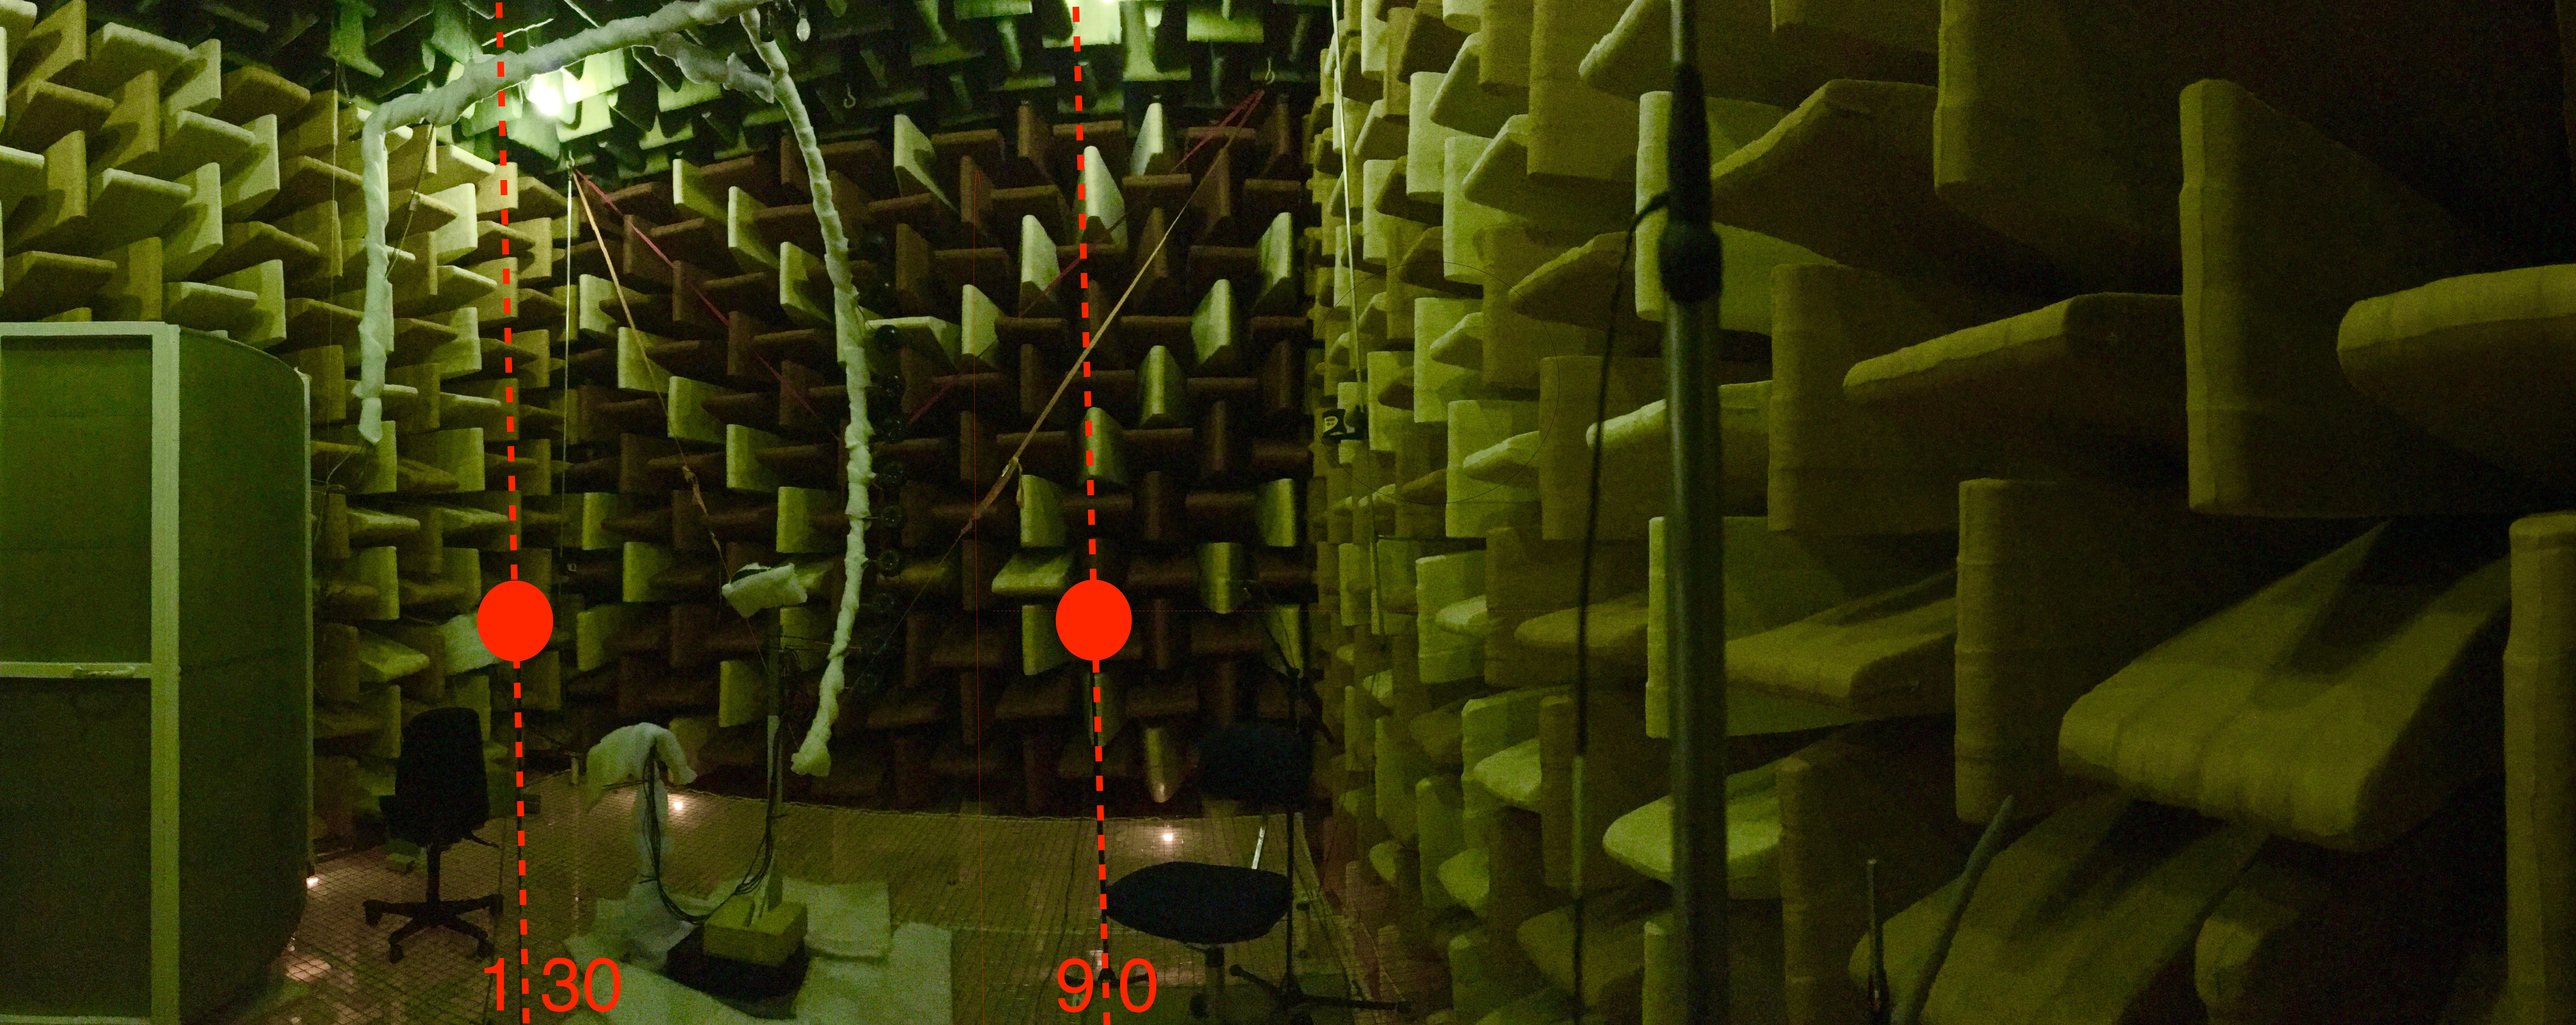
\includegraphics[width=1\textwidth]{Figures/AnechoicPic.jpg}
    \caption{Picture of the set up. The anechoic chamber was filled with misc. equipment, therefore the sources have been replaced by red dots for clarity. 90 and 130 $\degree$ azimuth are also drawn on top of the picture.}
    \label{fig:Anechoicpic1}
\end{figure}

\begin{figure}[H]
    \centering
    \includegraphics[width=0.7\textwidth]{Figures/Anechoicexp3.png}
    \caption{Diagram of the experiment}
    \label{fig:Anechoicexp3}
\end{figure}

\subsubsection{Results}

\begin{figure}[H]
    \centering
    \begin{subfigure}[b]{0.96\textwidth}
    \centering
    \includegraphics[width=0.95\textwidth]{Figures/Anechoic2SrcNorm.png}
\end{subfigure}
\vskip \baselineskip
\begin{subfigure}[b]{0.96\textwidth}
    \centering
    \includegraphics[width=0.95\textwidth]{Figures/Anechoic2SrcMinPow.png}
\end{subfigure}
\caption{Figures depict from top-to-bottom SRP-PHAT and minimum power SRP-PHAT localization}
\end{figure}

During the experiment, the anechoic chamber was not completely empty and some reflections can be observed at and below 12dB dynamic range, which potentially masks the secondary (lower magnitude) source. Also, since the speakers are relatively close to the array, the cone approximation has larger errors. This can reduce the size of overlap of the multiple cones from the various microphones. This can be seen in the result for normal SRP-PHAT here, where the cones for the secondary cones barely overlap. Minimum power SRP-PHAT can then completely hide the secondary source. Over here however, the secondary source can be just seen. 
%The maximum dynamic range achievable is correlated to the amount of reflections and noise in the environment, specially when localizing multiple sources. 
%For near free-field conditions with few reflections a dynamic range of 12dB can be achieved whereas very reflective environments will limit the dynamic range to 3dB in the worst case.

%
%\begin{figure}[H]
%    \centering
%    \begin{subfigure}[t]{0.5\textwidth}
%    \centering
%    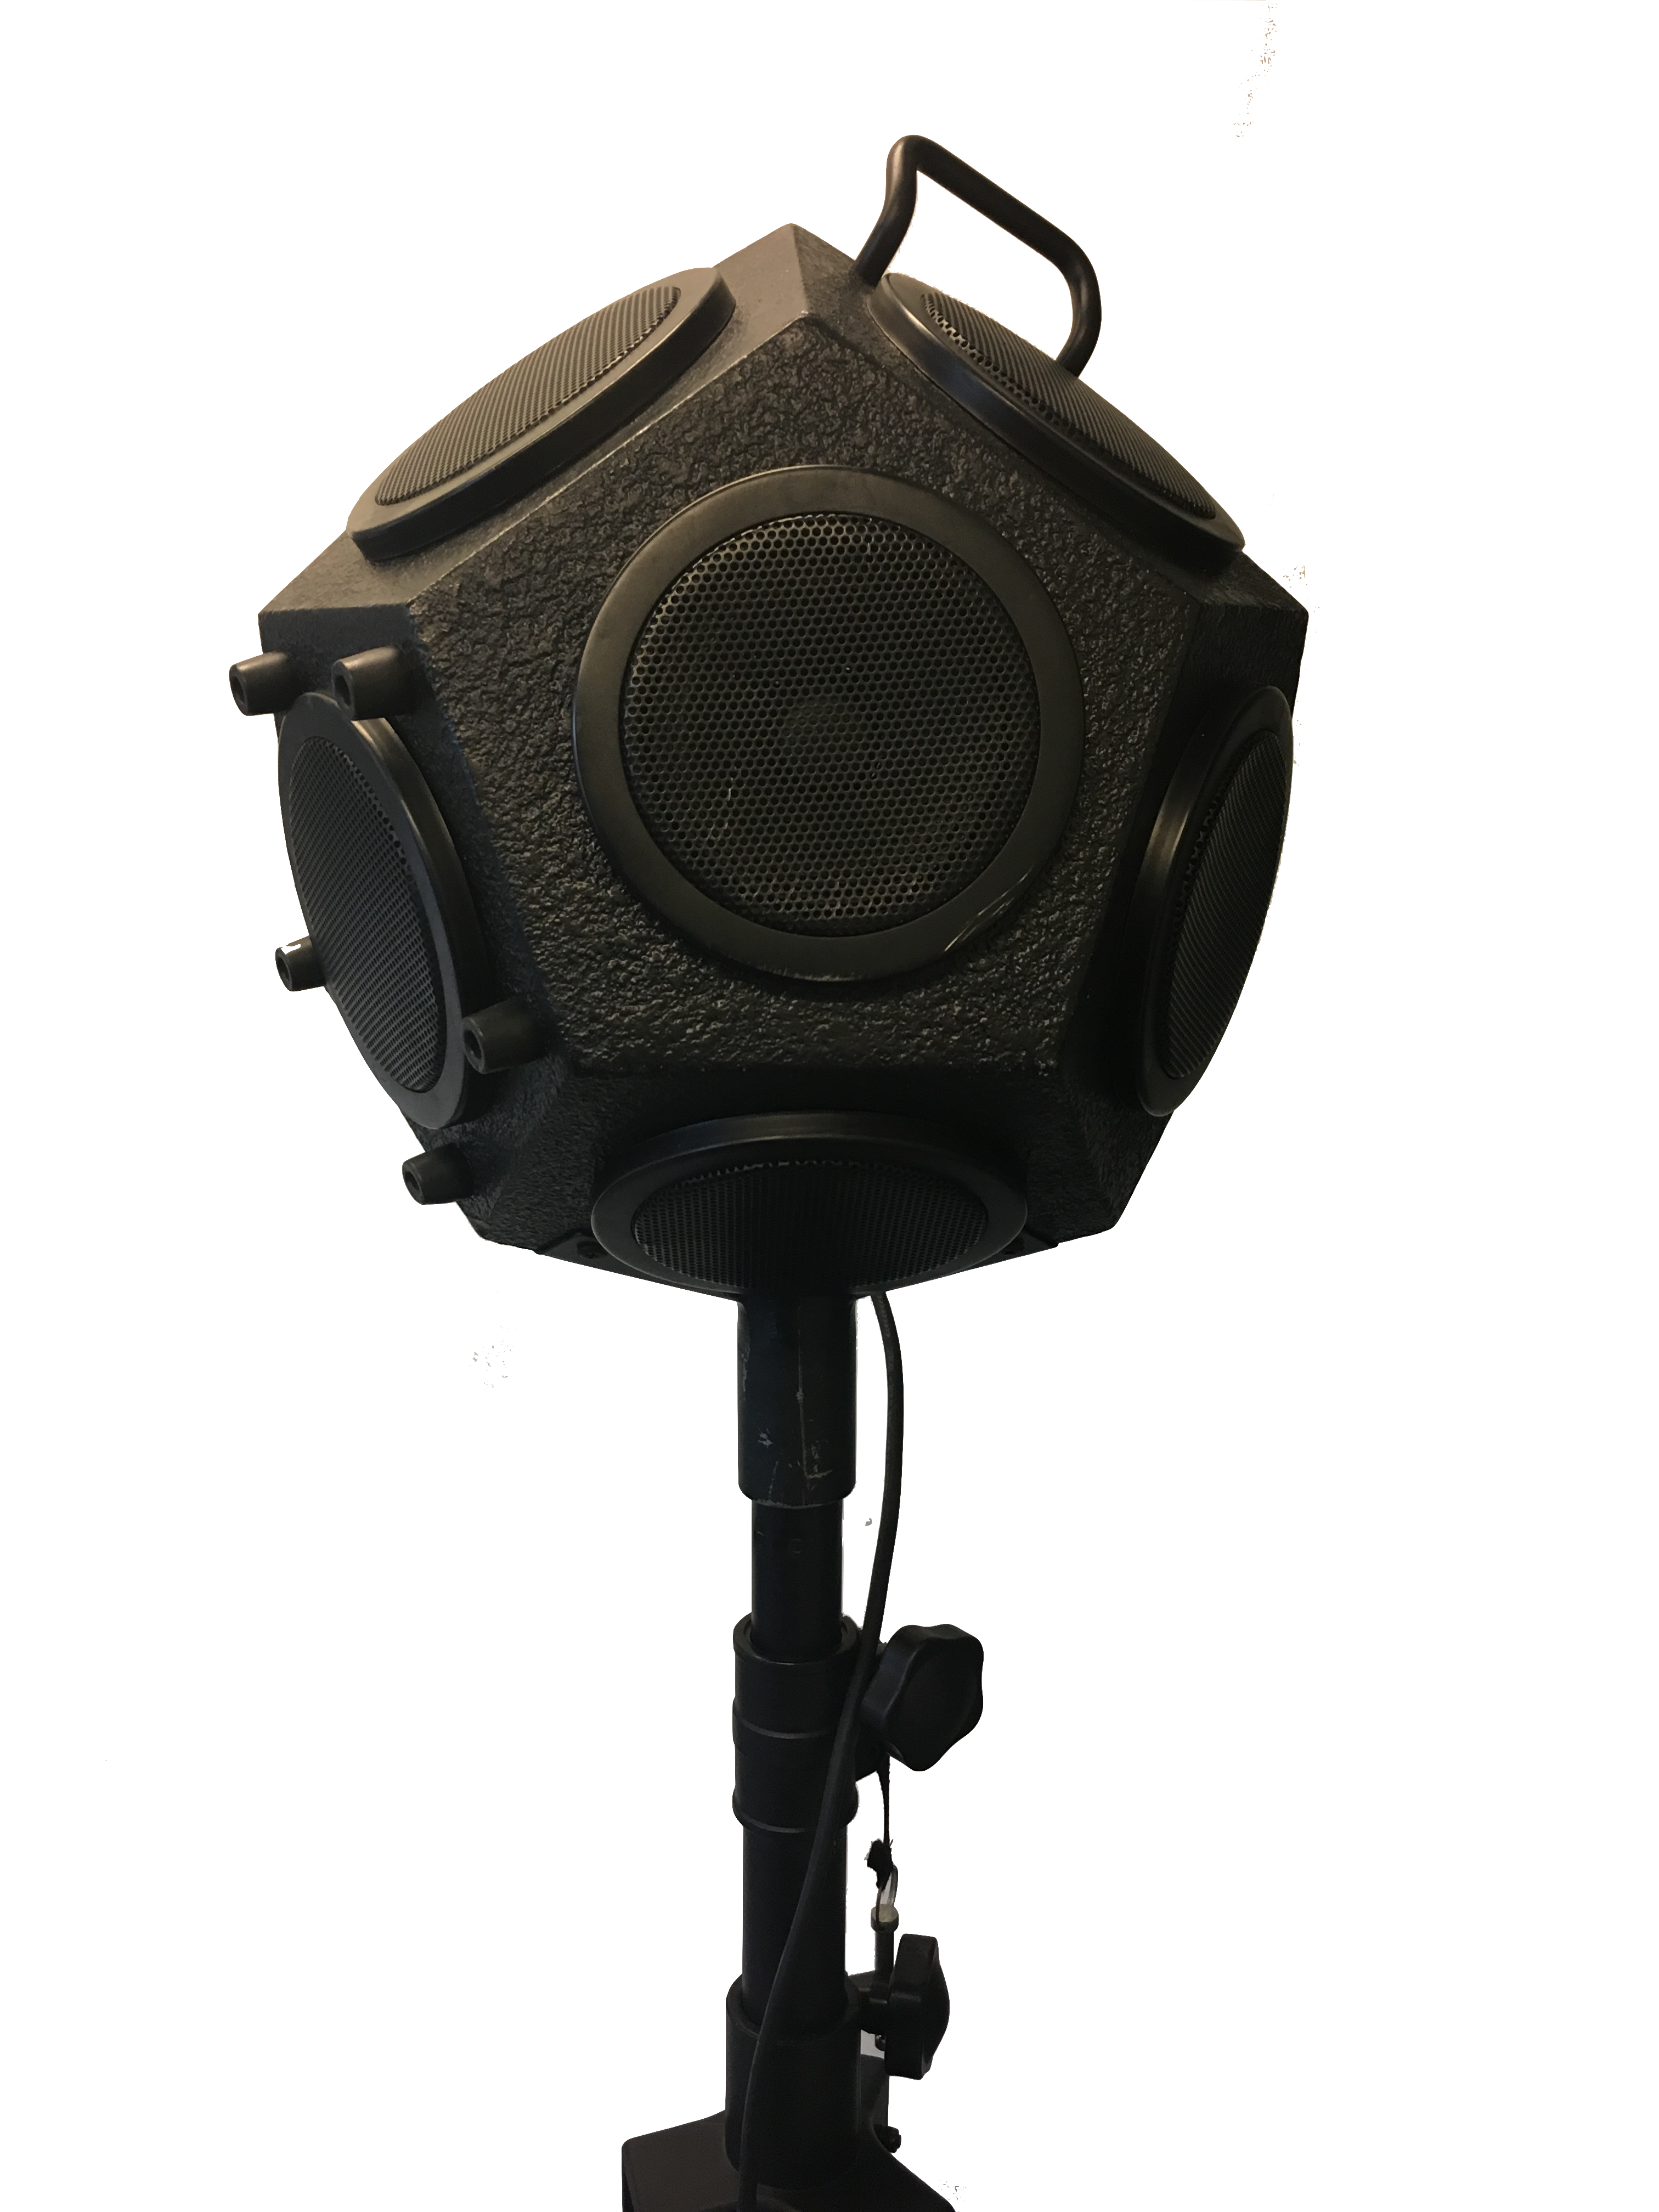
\includegraphics[width=0.9\textwidth]{Figures/IMG_7337.png}
%    \caption{B\&K Omnisource}
%    \label{fig:Omnisource}
%\end{subfigure}%
%\begin{subfigure}[t]{0.5\textwidth}
%        \centering
%    \includegraphics[width=0.9\textwidth]{Figures/Arraymicrophone.png}
%    \caption{Prototyped microphone array}
%    \label{fig:Array}
%\end{subfigure}
%\end{figure} 

\newpage

\section{Outdoor measurements}
In order to test the algorithm in real conditions, several outdoor measurements in various conditions are conducted, in a construction field, in concerts, in traffic and in a mining field. The recordings are done at the maximum sample rate available in the system, viz, 131072kHz. The microphone array aperture unless otherwise mentioned, is set at 1m, since the sources were always sufficiently far away. Pictures of the measured outdoor environment are taken using a camera with a known angle of view, to retrieve the azimuth and elevation. The localization results are then overlaid on the pictures.

\subsection{One static source on a construction field}

In this scenario, a single construction machine working in a fixed position is recorded by the microphone array. The source is more than 20 meters away. Fig. \ref{fig:Scenario1pic} describes the setup. The measurement system is set in the middle of a road, outside the construction field. Behind the setup is a big office building with a smooth faćade. Temperature is recorded at 23$\degree$C, speed of wind is 2m/s from (180$\degree$, 0$\degree$). Fig. \ref{Fig:OutdoorLast1Src} displays the results.

\begin{figure}[H]
    \centering
    \begin{subfigure}[b]{0.96\textwidth}
    \includegraphics[width=1\textwidth]{Figures/Scenario1pic.jpg}
    \end{subfigure}
    \vskip \baselineskip
    \begin{subfigure}[b]{0.8\textwidth}
    \includegraphics[width=0.8\textwidth]{Figures/scenario2diagram.png}
    \end{subfigure}
    \caption{Figure shows the picture of the construction field (top) and the top view schematic of the construction field (bottom)}
    \label{fig:Scenario1pic}
\end{figure}

\begin{figure}[H]
    \centering
    \begin{subfigure}[b]{0.96\textwidth}
    \centering
    \includegraphics[width=0.95\textwidth]{Figures/OutsideLastNorm.png}
\end{subfigure}
\vskip \baselineskip
\begin{subfigure}[b]{0.96\textwidth}
    \centering
    \includegraphics[width=0.95\textwidth]{Figures/OutsideLastMinPow.png}
\end{subfigure}
\caption{Figures depict from top-to-bottom SRP-PHAT and minimum power SRP-PHAT localization}
\label{Fig:OutdoorLast1Src}
\end{figure}

The recordings are 51sec long. Since the recordings used to localize are of a relatively long duration, short-timed or spontaneous sound events would not appear as high on the map, since they are effectively averaged out. The results are shown in figure \ref{Fig:overlayimageoutside2}. Even though the machine itself does not move, the excavator arm moves around the body of the machine, and as can be seen, the sounds emitted at different positions around the motor due to the arm do not appear as much on the result image. The dynamic range of the map has been adjusted to filter out the reflections and less powerful sources. Results for dynamic range of 12dB and 6dB are shown. It is indeed difficult to get a clean map for a large dynamic range, as more and more reflections from the source become apparent, as well as other distant sources and their own reflections. In addition, other noise sources such as the wind or other diffuse reflections can appear on the results.

\begin{figure}[H]
    \centering
    \begin{subfigure}[b]{0.96\textwidth}
    \centering
    \includegraphics[width=1\textwidth]{Figures/Outside2MinPow12dB.png}
\end{subfigure}
\vskip \baselineskip
\begin{subfigure}[b]{0.96\textwidth}
    \centering
    \includegraphics[width=1\textwidth]{Figures/Outside2MinPow6dB.png}
\end{subfigure}
\caption{Figures depict localization results overlaid on the measured source picture with dynamic range of 12dB (top) and 6dB (bottom)}
\label{Fig:overlayimageoutside2}
\end{figure}

\newpage
\subsection{3 static sources on a construction field}

In this scenario, 3 distinct noise sources are present: 1 tapping machine, in a hole in the ground, located at (180$\degree$,<0$\degree$) and two excavators located at around (120$\degree$-150$\degree$,0$\degree$). Fig. \ref{fig:Scenario2} describes the setup. Fig. \ref{Fig:Outdoorpicfull} displays the results.

\begin{figure}[H]
    \centering
    \begin{subfigure}[b]{0.96\textwidth}
    \includegraphics[width=1\textwidth]{Figures/scenario3pic.jpg}
    \end{subfigure}
    \vskip \baselineskip
    \begin{subfigure}[b]{0.96\textwidth}
    \centering
    \includegraphics[width=1\textwidth]{Figures/scenario1diagram.png}
    \end{subfigure}
    \caption{Panorama of the construction field at the center point of the microphone array (top) and Top view schematic of the construction field (bottom)}
    \label{fig:Scenario2}
\end{figure}

\begin{figure}[H]
    \centering
    \begin{subfigure}[b]{1\textwidth}
    \centering
     \includegraphics[width=1\textwidth]{Figures/Scenario1DYN6.png}
\end{subfigure}
\vskip \baselineskip
\begin{subfigure}[b]{1\textwidth}
    \centering
    \includegraphics[width=1\textwidth]{Figures/Scenario1DYN3.png}
\end{subfigure}
\caption{Figures depict from top-to-bottom Min SRP-PHAT with dynamic range of 6dB and 3dB}
\label{Fig:Outdoorpicfull}
\end{figure}
\begin{figure}[H]
\vskip \baselineskip
\begin{subfigure}[b]{1\textwidth}
    \centering
    \includegraphics[width=1\textwidth]{Figures/Scenario1DYN3Zoomed.png}
\end{subfigure}
\caption{Zoomed figure depict from top-to-bottom Min SRP-PHAT with dynamic range of 3 dB}
\label{Fig:Outdoorpicfull}
\end{figure}

\newpage
\subsection{Sport event with crowd and PA system }

Measurements are performed during a sport competition outside, two main noise sources are present. The first one is a distributed PA system that covers all the zone as shown in figure \ref{fig:Scenario1diagram}, the second one is a crowd at (0°,0°).

\begin{figure}[H]
    \centering
    \includegraphics[width=1\textwidth]{Figures/bmxracepic.jpg}
    \caption{Panorama of the setup at the center point of the microphone array}
    \label{fig:Scenario3}
\end{figure}

\begin{figure}[H]
    \centering
    \includegraphics[width=0.8\textwidth]{Figures/bmxrace1.png}
    \caption{Top view of the scenario}
    \label{fig:Scenario1diagram}
\end{figure}

\begin{figure}[H]
    \centering
    \begin{subfigure}[b]{1\textwidth}
    \centering
    \includegraphics[width=1\textwidth]{Figures/BMX_1_6.png}
\end{subfigure}
\vskip \baselineskip
\begin{subfigure}[b]{1\textwidth}
    \centering
    \includegraphics[width=1\textwidth]{Figures/BMX_1_3.png}
\end{subfigure}
\caption{Figures depict from top-to-bottom Min SRP-PHAT with dynamic range of 6dB and 3dB}
\label{Fig:bmxracedyn}
\end{figure}

\begin{figure}[H]
    \centering
    \begin{subfigure}[b]{1\textwidth}
    \centering
    \includegraphics[width=1\textwidth]{Figures/BMX_1_6_zoomed.png}
\end{subfigure}
\vskip \baselineskip
\begin{subfigure}[b]{1\textwidth}
    \centering
    \includegraphics[width=1\textwidth]{Figures/BMX_1_3_zoomed.png}
\end{subfigure}
\caption{Figures depict from top-to-bottom Min SRP-PHAT with dynamic range of 6dB and 3dB}
\label{Fig:bmxracezomm}
\end{figure}

\newpage
\subsection{Outdoor concert}
Measurements are performed during an outdoor concert in a free-field condition, a DJ is playing music on a Public Address system. The PA system is composed of two tops and one sub. The setup can be seen in figure \ref{fig:Scenario4}

\begin{figure}[H]
    \centering
    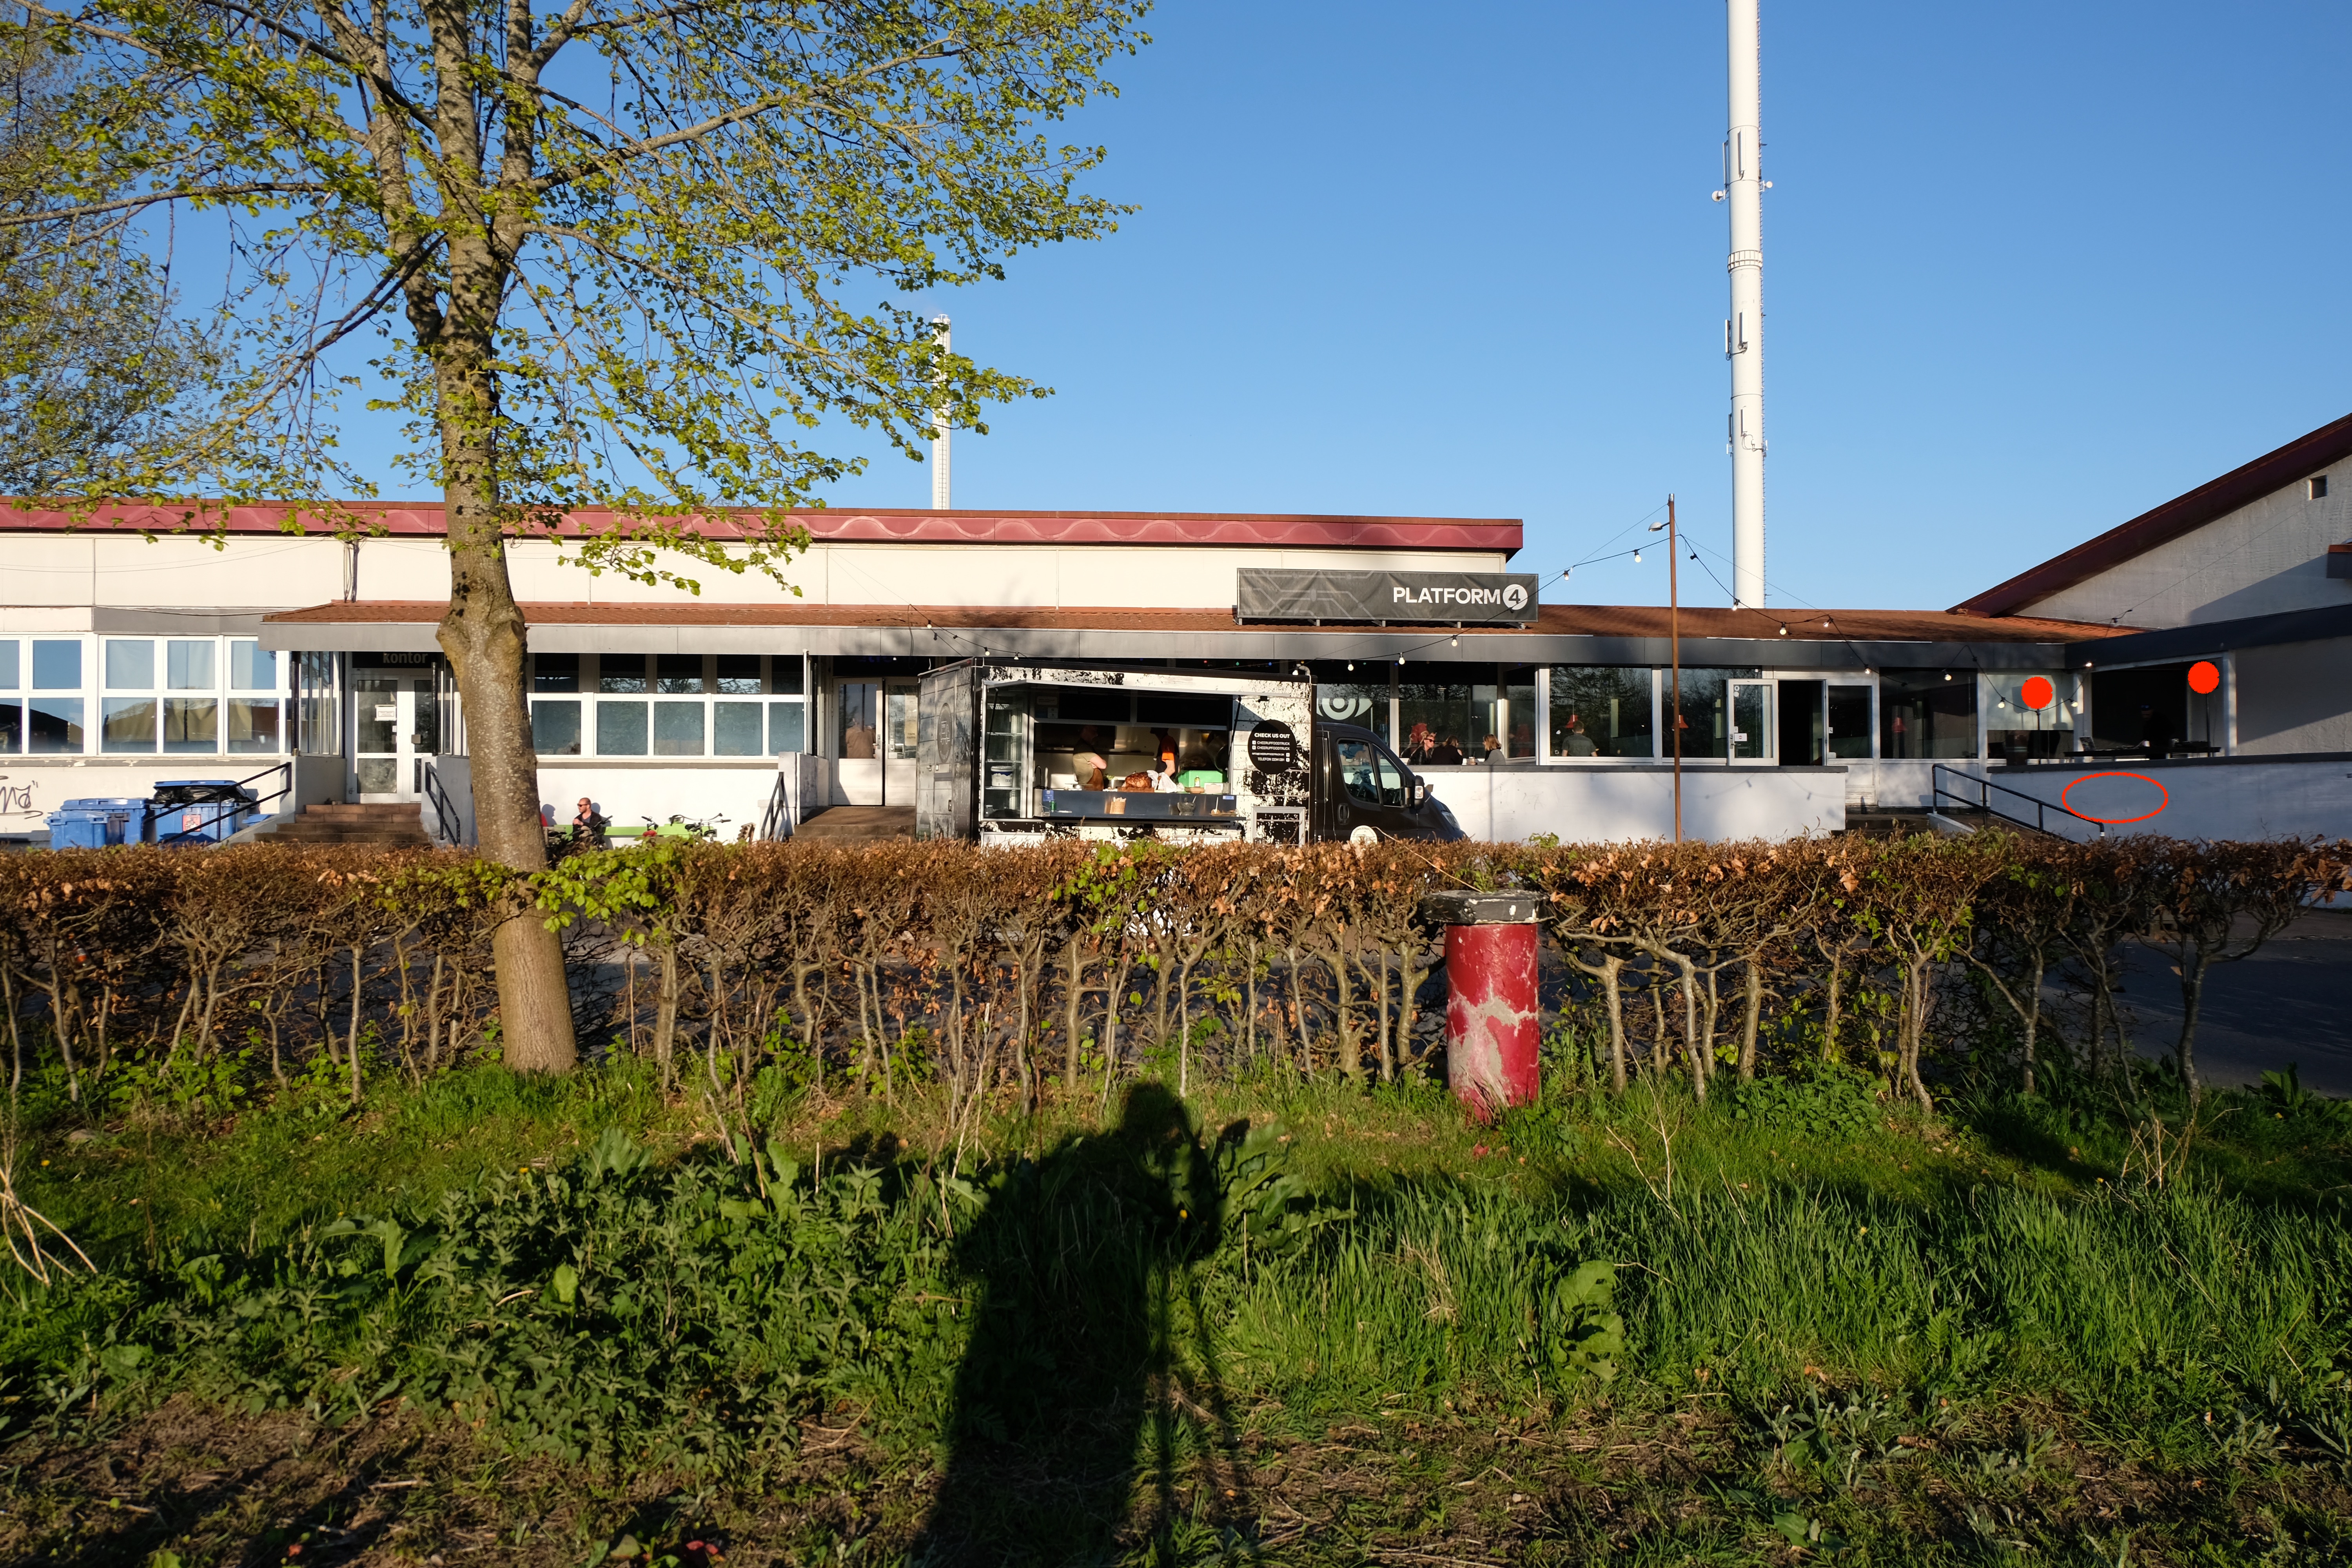
\includegraphics[width=1\textwidth]{Figures/P4day.jpg}
    \caption{Picture of the setup at the center point of the microphone array}
    \label{fig:Scenario4}
\end{figure}

\begin{figure}[H]
    \centering
    \begin{subfigure}[b]{1\textwidth}
    \centering
    \includegraphics[width=1\textwidth]{Figures/P4_Day_6.png}
\end{subfigure}
\vskip \baselineskip
\begin{subfigure}[b]{1\textwidth}
    \centering
    \includegraphics[width=1\textwidth]{Figures/P4_Day_3.png}
\end{subfigure}
\caption{Figures depict from top-to-bottom Min SRP-PHAT with dynamic range of 6dB and 3dB(Zoomed)}
\label{Fig:P4Day}
\end{figure}

\subsection{Indoor concert}
Measurements are made of a concert happening indoors.

\begin{figure}[H]
    \centering
    \begin{subfigure}[b]{1\textwidth}[H]
    \centering
    \includegraphics[width=1\textwidth]{Figures/P4Night6dB.png}
\end{subfigure}
\vskip \baselineskip
\begin{subfigure}[b]{1\textwidth}[H]
    \centering
    \includegraphics[width=1\textwidth]{Figures/P4Night3dB_Zoomed.png}
\end{subfigure}
\caption{Figures depict from top-to-bottom Min SRP-PHAT with dynamic range of 6dB and 3dB(Zoomed)}
\label{Fig:P4Night}
\end{figure}

\subsection{Roadside noise}
Cars passing through a crossing are measured in a close range ($2-10m$). A single loud motorcycle passing through is measured.

\subsubsection{General traffic}

\subsubsection{Loud motorcycle}

\subsection{Chalk mine}
A chalk mining machine is measured from a large distance ($500m$), with different microphone aperture sizes. The same measurement is then run closer ($100m$) and even closer ($90m$).
\subsubsection{Lookout large aperture}
\begin{figure}[H]
    \centering
    \includegraphics[width=1\textwidth]{Figures/ChalkFarFar.png}
    \caption{Localization results of the chalk mine from a far away lookout close to traffic noise}
    \label{fig:ChalkCLose}
\end{figure}

%\subsubsection{Lookout small aperture}

\subsubsection{Close to mine, far from edge}
\begin{figure}[H]
    \centering
    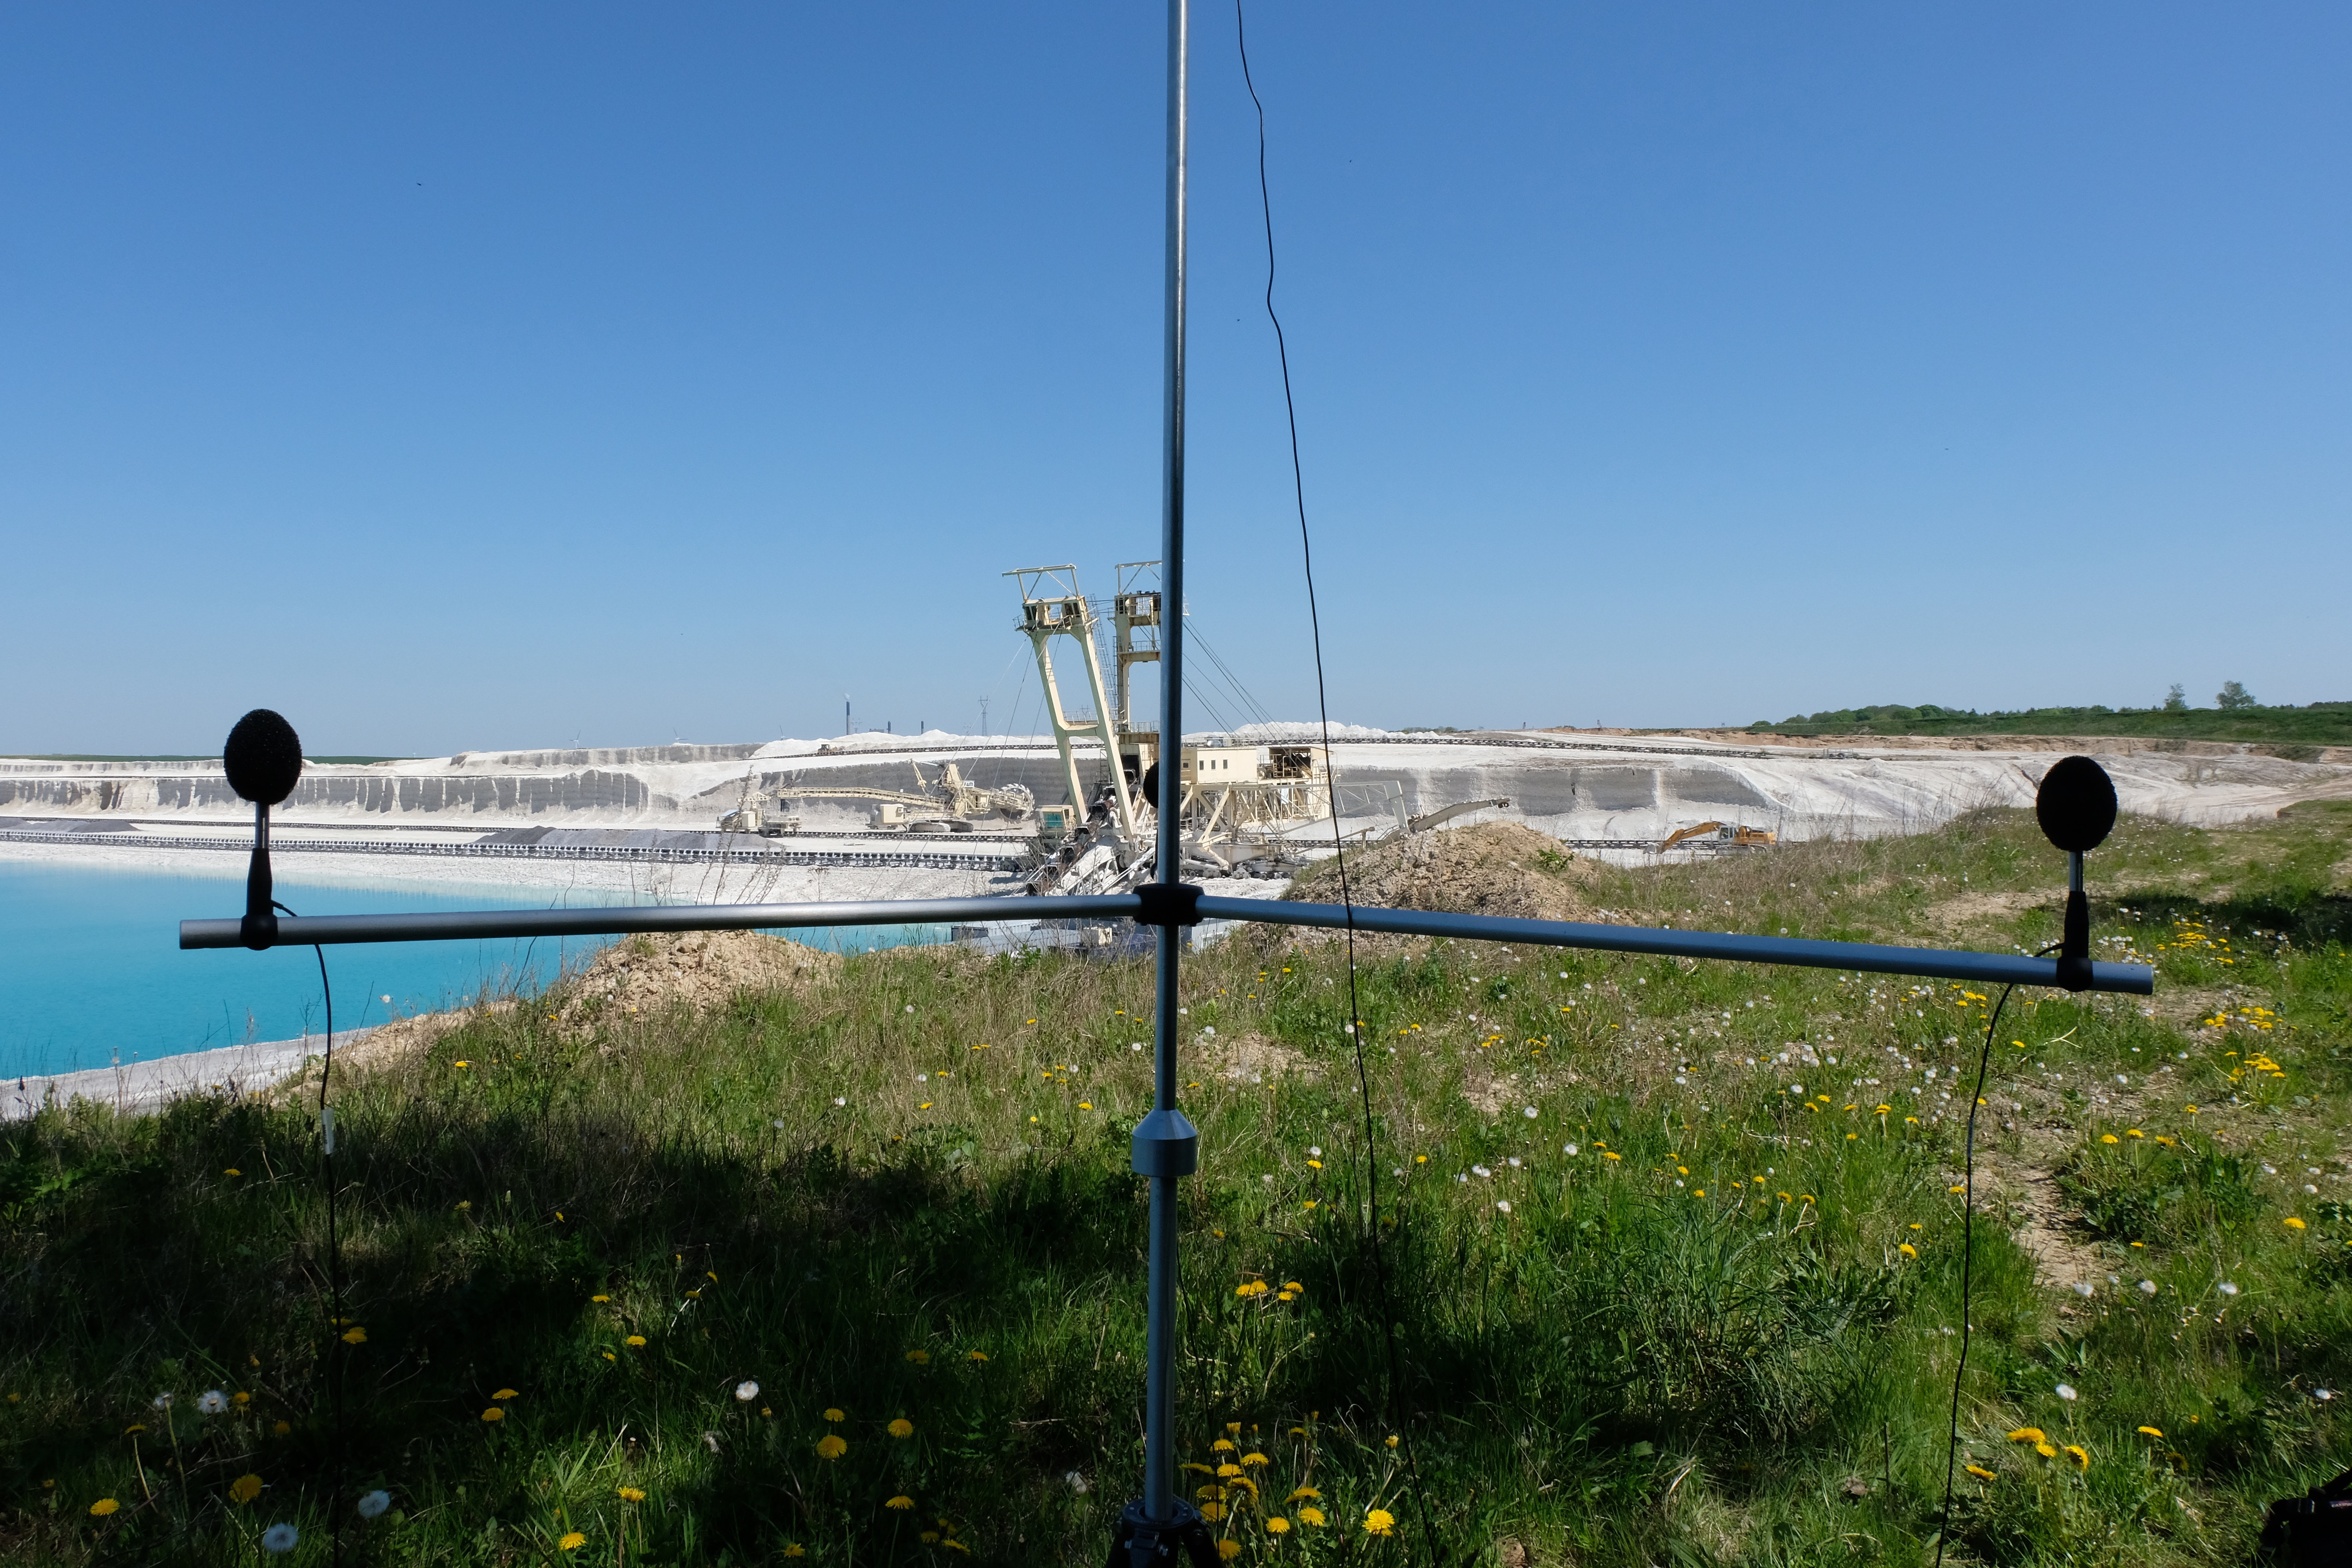
\includegraphics[width=1\textwidth]{Figures/ChalkFar.png}
    \caption{Localization results of the chalk mine far from the edge}
    \label{fig:ChalkCLose}
\end{figure}

\subsubsection{Close to mine, close to edge}

\begin{figure}[H]
    \centering
    \includegraphics[width=1\textwidth]{Figures/ChalkClose.png}
    \caption{Localization results of the chalk mine close to the edge}
    \label{fig:ChalkCLose}
\end{figure}

\subsubsection{Length of recording}

\begin{figure}[H]
\begin{subfigure}[b]{0.96\textwidth}
    \centering
    \includegraphics[width=0.8\textwidth]{Figures/ChalkCloseFull1Sec.png}
\end{subfigure}
\vskip \baselineskip
\begin{subfigure}[b]{0.96\textwidth}
    \centering
    \includegraphics[width=0.8\textwidth]{Figures/ChalkCloseFull10Sec.png}
\end{subfigure}
\vskip \baselineskip
\begin{subfigure}[b]{0.96\textwidth}
    \centering
    \includegraphics[width=0.8\textwidth]{Figures/ChalkCloseFull120Sec.png}
\end{subfigure}
\caption{Figures depict from SRP-PHAT localization results, for recording length 1sec (top), 10sec (middle) and 120sec (bottom)}
\label{fig:4mic1srcRedun}
\end{figure}

